%!TEX root=main.tex
\subsubsection{Definiciones previas}
En base al estudio de los distintos diseños de alcuza disponibles en el mercado se clasificaron los diseños en 2 tipos principales: tradicional y no tradicional. Los cuales se definen a continuación.

\textbf{Tradicional:} Se entiende por un diseño tradicional aquel que está compuesto por botellas de vidrio o cerámica, de color transparente o monocromático con tapa de madera,  vidrio o metal. En adición puede poseer una bombilla adaptada.

\textbf{No tradicional:} Un diseño no tradicional será todo aquel diseño que no se clasifica como tradicional. De acuerdo a aquello esta variante posee alguna característica innovadora respecto del modelo clásico dominante. Entre ellas se pueden mencionar una adaptación diferente para aplicar el contenido, diseño en la pintura o forma  creativa.

En  cuanto a la definición del cliente final de las alcuzas, la investigación que se muestra en siguiente inciso permitió determinar dos tipos:

\textbf{Clientes tipo 1:} personas que compran una alcuza para su casa o para regalo.

\textbf{Clientes tipo 2:} restaurantes que compran alcuzas para su negocio.

\subsubsection{Demanda: Levantamiento de información}

En la actualidad el registro de datos públicos acerca de la demanda de alcuzas es nulo. No existe información detallada sobre la participación de mercado de cada una, ni sobre el volumen que ofertan las empresas que venden este producto. Por dicha razón, se utilizaron distintas metodologías para estimar los datos faltantes, en específico se realizaron entrevistas y encuestas, las cuales se detallan a continuación.

\begin{itemize}
\item \textbf{Entrevistas a tiendas comerciales:}
\end{itemize}

Las entrevistas se realizaron con los siguientes objetivos: conocer la cantidad de alcuzas vendidas al mes; identificar proveedores; averiguar qué diseños que tienen a la venta y sus respectivos ciclos de vida en la tienda; e indagar sobre las principales características de las personas que compran alcuzas.

Hasta el momento se han entrevistado 6 tiendas distintas, Paris, Falabella, Ripley, Casa\&Ideas, Kitchen Republic y Capdor. Cabe mencionar que la totalidad de las tiendas estaban ubicadas en el Mall Costanera Center.

En el Anexo \ref{PauEntRetail} se detalla la pauta de preguntas que se utilizó. Dicha guía está sujeta a flexibilidades, dado que cada entrevista se orientó según variaciones surgidas en el momento.

Las respuestas obtenidas permiten concluir que el perfil general de clientes que compran alcuzas es variado. Se identificaron los siguientes motivos de compra: adquisición para luego regalarla, realizar una reposición o al momento de mudarse a una casa nueva. En cuanto a tasa de ventas, se determinó que la tienda Falabella vende alrededor de 15 alcuzas al mes durante noviembre y diciembre, y el resto del año vende aprox. 5 alcuzas al mes. Las tiendas Kitchen Republic y Casa\&ideas venden 40 y 20 unidades mensuales, respectivamente.  La tienda Capdor vende entre 15 y 20 alcuzas al mes. En adición, según estimaciones de la vendedora entrevistada de Falabella, la proporción de ventas de alcuzas tradicionales y no tradicionales es 8:2. En el Anexo \ref{ResEntRetail} se muestra la información de forma detallada.

Durante las visitas a tiendas comerciales se investigaron las marcas o fábricas y los países de fabricación de las alcuzas. En el Anexo \ref{MarAlc} se muestra la lista obtenida.



\begin{itemize}
\item \textbf{Entrevistas a restaurantes:}
\end{itemize}

Las entrevistas se realizaron con el objetivo de conocer la cantidad de alcuzas que poseen los restaurantes en relación a la cantidad de mesas, determinar cuántas veces al año realizan reposición de alcuzas, averiguar cuales son sus proveedores de alcuzas y de aceite, obtener una aproximación del dinero que están dispuestos a pagar por una alcuza y, por último, percibir opiniones acerca del diseño que se está evaluando y conocer disposición a pagar por este.

En el Anexo \ref{PauEntRest} se detalla la pauta seguida en estas entrevistas, hasta el momento se han entrevistado 12 restaurantes, 10 ubicados en Providencia y 2 en Isla de Maipo. Los locales entrevistados fueron: Barandiara, Parrillada del Chef, Voraz, Sandwicheria \& Bistro, Diddlers Irish Bar \& Restaurant, Le Fournil, Luca’s, My Tavuk, Shopdog, Normandie, El Rincón Rústico y Ziufande.


Las entrevistas permitieron concluir que aquellos restaurantes que forman parte de una cadena o franquicia no compran alcuzas, sino que sus proveedores se las regalan o venden a un mejor precio. Por otro lado, la porción de restaurantes que si compran alcuzas prefiere diseños tradicionales  frente al diseño de alcuza integrada. Entre las razones que mencionaron fue que poseen un diseño de alcuza fijo en el local y realiza compra para reponer su \textit{stock} de alcuzas, y un diseño no tradicional implica educar al cliente acerca de su uso.

En cuanto a datos cuantitativos, se determinó que cada restaurante posee aproximadamente 1 alcuza por mesa y que se realiza reposición de alcuzas una vez al año. En el Anexo \ref{ResResEntRest} se muestra una tabla resumen de los Resultados de las entrevistas. En forma adicional, en el Anexo \ref{ResEntRest} se muestran las respuestas de cada restaurante de forma detallada.

\begin{itemize}
\item \textbf{Encuestas a personas:}
\end{itemize}

Los principales objetivos de la encuesta son: obtener una estimación de la demanda de alcuzas en general; indagar si las personas conocen el producto y lo utiliza en su casa a diario; determinar el perfil de los posibles compradores del producto; conocer su comportamiento de compra y preferencias; y averiguar la disposición a comprar el diseño de alcuza integrada.

Las encuestas se realizaron en el camino entre la estación de metro Tobalaba y el centro comercial Mall Costanera Center, entre las 15:00 y 18:30 hrs. durante un día domingo. Cabe destacar que el sondeo abarcó a 57 personas.  En el  Anexo \ref{PauEnc} se detallan las preguntas realizadas. Para la posterior utilización de los datos se supuso que cada persona entrevistada representó a un hogar, debido a que el producto estudiado está presente en forma unitaria en las casas, esta última información se corroboró al momento de realizar la encuesta.

Las encuestas permitieron determinar que el 57,9\% de los encuestados poseen una alcuza en su casa. El 35,1\% de las personas encuestadas utiliza a diario la alcuza al momento de comer. En cuanto al comportamiento de compra se concluyó que el 33,4\% compró una alcuza hace menos de 3 años y el 26,4\% compró una alcuza durante el año 2016. En el Anexo \ref{ResEncPer}  se muestran las respuestas tabuladas.


\begin{itemize}
\item \textbf{Entrevistas a empresas de aceite:}
\end{itemize}

Los objetivos de las entrevistas a empresas productoras de aceite son: indagar acerca de sus proveedores de envases de vidrio, conocer la cantidad de envases de vidrio que compra la empresa mensualmente, determinar si la organización es proveedor directa de restaurantes, averiguar si la empresa cuenta con el servicio de venta o regalo de alcuzas a sus clientes y conocer la forma en que producen o compran las alcuzas.

Las organizaciones entrevistadas fueron Las Doscientas y Olivos Ruta del Sol, la primera fue realizada presencialmente mientras que la segunda se realizó mediante correo electrónico. En el Anexo \ref{PauEntEmpAce} se muestra la pauta de preguntas realizadas.

De las dos empresas entrevistadas, una empresa es proveedora directa de aceite de oliva a restaurantes, además posee su propio diseño de alcuza, el cual  vende a cierta cantidad de restaurantes en forma exclusiva. En adición se averiguó que el proveedor de envases de vidrio de ambas empresas es Cristalerías Toro. En el Anexo \ref{ResEntEmpAce} se muestran las respuestas detalladas de las entrevistas.

Cabe destacar que las entrevistas y encuestas sirvieron como una primera aproximación al mercado, y en el futuro se espera realizar más indagaciones de la misma forma que aporten mayor solidez a los datos obtenidos.

\subsubsection{ Participación de mercado}

Para determinar la participación de mercado se realizó el cálculo del porcentaje de ventas que corresponde a alcuzas tradicionales, para ello se utilizaron los datos obtenidos en las entrevistas a tiendas comerciales. Aquello permitió determinar qué aprox. el 80\% de las alcuzas vendidas corresponden a alcuzas de diseño tradicional y el resto no tradicional (esto para el caso de los locales que venden ambos tipos de diseño).

Se utilizó la venta mensual de alcuzas obtenida mediante de las entrevistas a tiendas comerciales, luego este dato se amplificó por la cantidad de sucursales que posee dicha tienda en la Región Metropolitana. Con ello se obtuvo una venta escalada a la región. Luego se determinó la cantidad total de ventas de alcuza tradicional con la suma ponderada de las ventas de la región con el 80\% correspondiente a porcentaje de alcuzas tradicionales a la venta. La cantidad total de ventas de alcuza no tradicional se calculó de forma similar, pero esta vez se ponderó la venta total por 20\%, correspondiente a las ventas de alcuzas no tradicionales. La Tabla \ref{PartMercAlcu} muestra los datos utilizados y resultados obtenidos.

\begin{table}[H]
\centering
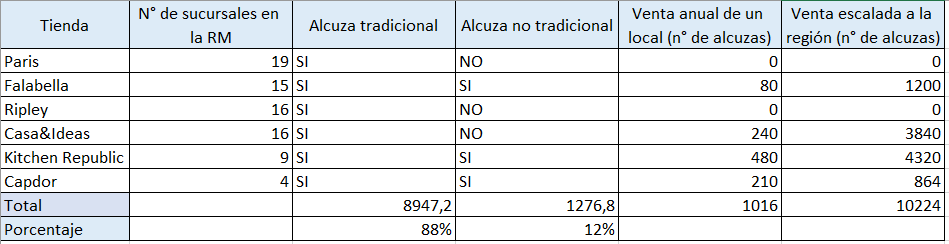
\includegraphics[width=\textwidth]{PartMercAlcu.png}
\caption{Participación de mercado de alcuzas, con datos obtenidos mediante entrevistas a tiendas.}
\label{PartMercAlcu}
\end{table}
